\documentclass[]{article}

% Imported Packages
%------------------------------------------------------------------------------
\usepackage{amssymb}
\usepackage{amstext}
\usepackage{amsthm}
\usepackage{amsmath}
\usepackage{enumerate}
\usepackage{fancyhdr}
\usepackage[margin=1in]{geometry}
\usepackage{graphicx}
\usepackage{extarrows}
\usepackage{setspace}
%------------------------------------------------------------------------------

% Header and Footer
%------------------------------------------------------------------------------
\pagestyle{plain}  
\renewcommand\headrulewidth{0.4pt}                                      
\renewcommand\footrulewidth{0.4pt}                                    
%------------------------------------------------------------------------------

% Title Details
%------------------------------------------------------------------------------
\title{Deliverable \#3 Template}
\author{SE 3A04: Software Design II -- Large System Design}
\date{}                               
%------------------------------------------------------------------------------

% Document
%------------------------------------------------------------------------------
\begin{document}

\maketitle
\noindent{\bf Tutorial Number:} T03\\
{\bf Group Number:} G06 \\
{\bf Group Members:}
\begin{itemize}
	\item Virochaan Ravichandran Gowri
	\item Alex Yoon
	\item Noah Goldschmied
	\item Krish Dogra
	\item Leo Vugert
\end{itemize}

\newpage
\section{Introduction}
\label{sec:introduction}
% Begin Section

\subsection{Purpose}
\label{sub:purpose}
% Begin SubSection
This document provides a more detailed look into the implementation details of the VanklComm application. The document contains state chart diagrams, sequence diagrams, and a detailed class diagram of the system. \\
\\The intended audience of the document are the stakeholders of VanklComm, which includes the developers, managers, investors, and any domain experts used for consulting. Deliverables 1 and 2 should be read prior to this document to ensure proper context for the project, and some technical knowledge is beneficial in order to properly read the diagrams seen in this document.
% End SubSection

\subsection{System Description}
\label{sub:system_description}
% Begin SubSection
An in depth overview of the system can be found in Deliverable 2. This document is a supplementary to Deliverable 2, and it provides more details to the system in the form of state charts, sequence diagrams and a class diagram.
% End SubSection

\subsection{Overview}
\label{sub:overview}
% Begin SubSection
This document containts many types of charts/diagrams. In section 2, there are state chart diagrams for every controller class that is found in the ACD in Deliverable 2. In section 3, there are relevant sequence diagrams to the system, and in section 4 there is a detailed class diagram which describes the architecture of the system.

% End SubSection

% End Section

\section{State Charts for Controller Classes}
\label{sec:state_charts_for_controller_classes}
% Begin Section
\begin{center}
	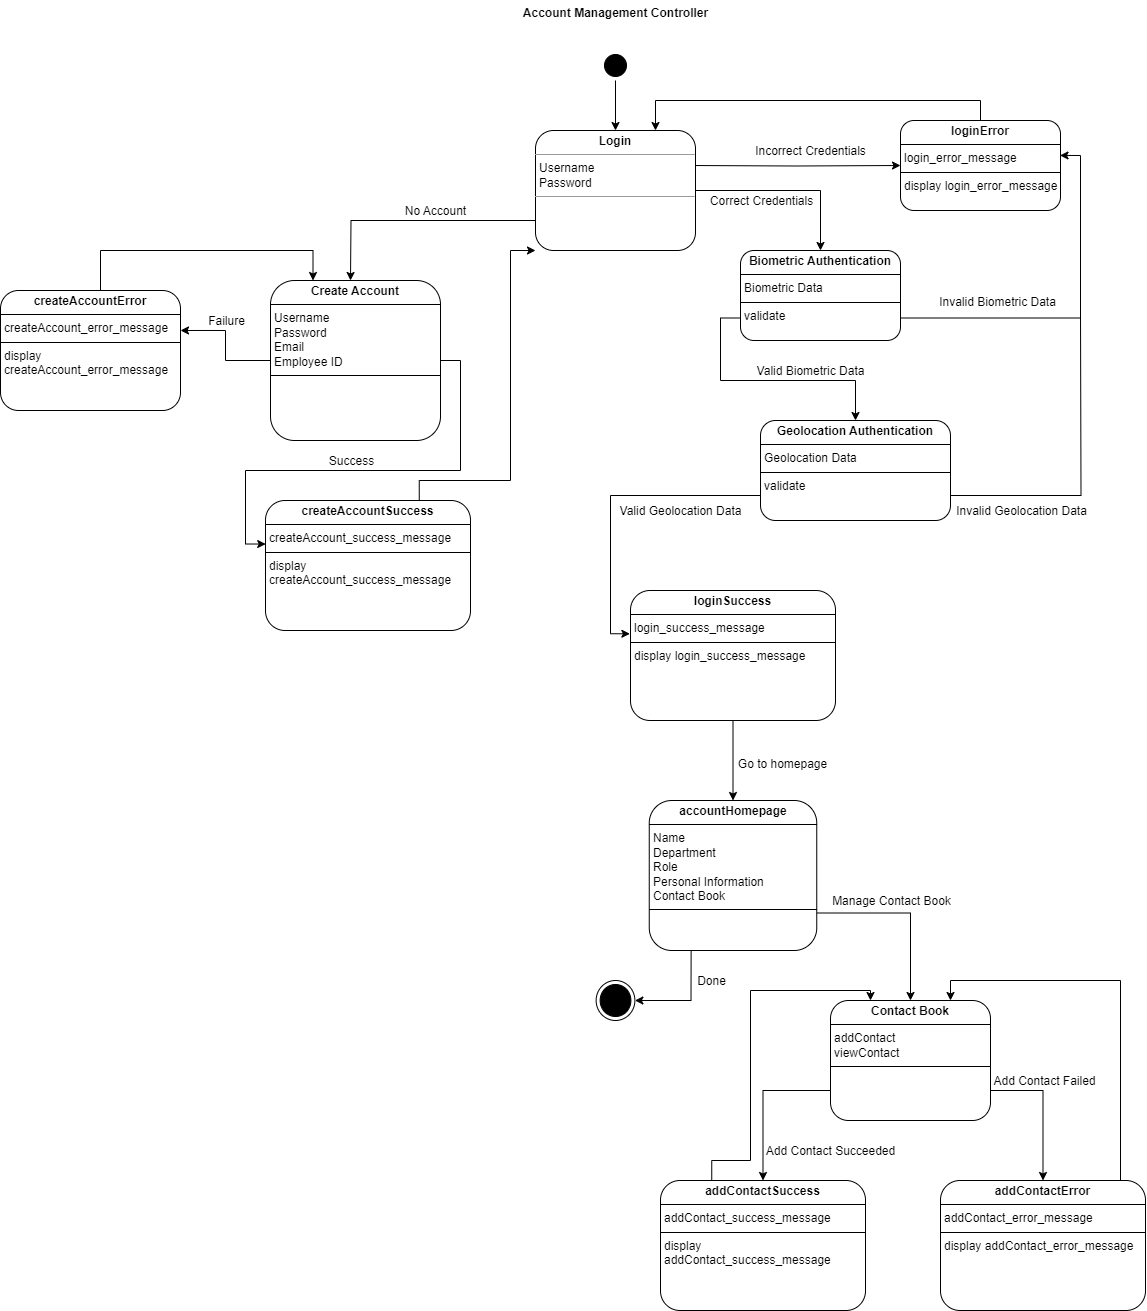
\includegraphics[width=\textwidth]{../images/ControllerStateDiagrams/AccountManagementController.drawio.png}
	\textbf{Figure 2.1 Overall Account Management Controller State Diagram}
	\\A more zoomed in view can be found in figures 2.1.1, 2.1.2, and 2.1.3.
	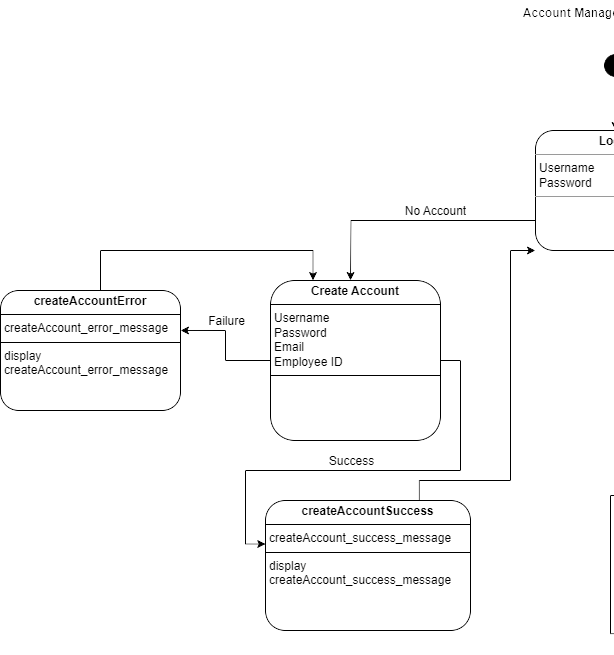
\includegraphics{../images/ControllerStateDiagrams/AMCTopLeft.png}
	\textbf{Figure 2.1.1 Top Left of the Account Management Controller State Diagram}
	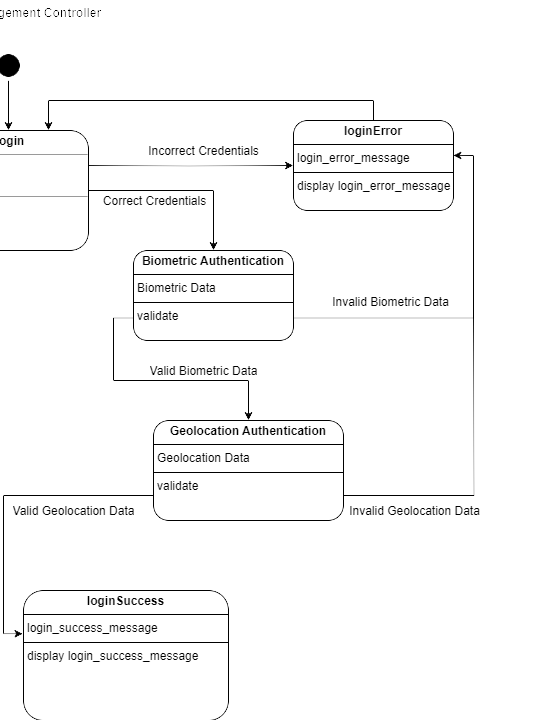
\includegraphics{../images/ControllerStateDiagrams/AMCTopRight.png}\\
	\textbf{Figure 2.1.2 Top Right of the Account Management Controller State Diagram}
	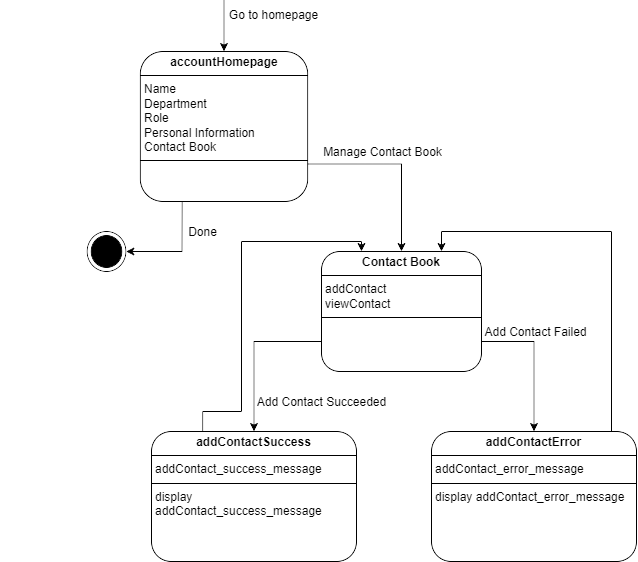
\includegraphics{../images/ControllerStateDiagrams/AMCBottom.png}
	\textbf{Figure 2.1.3 Bottom of the Account Management Controller State Diagram}

	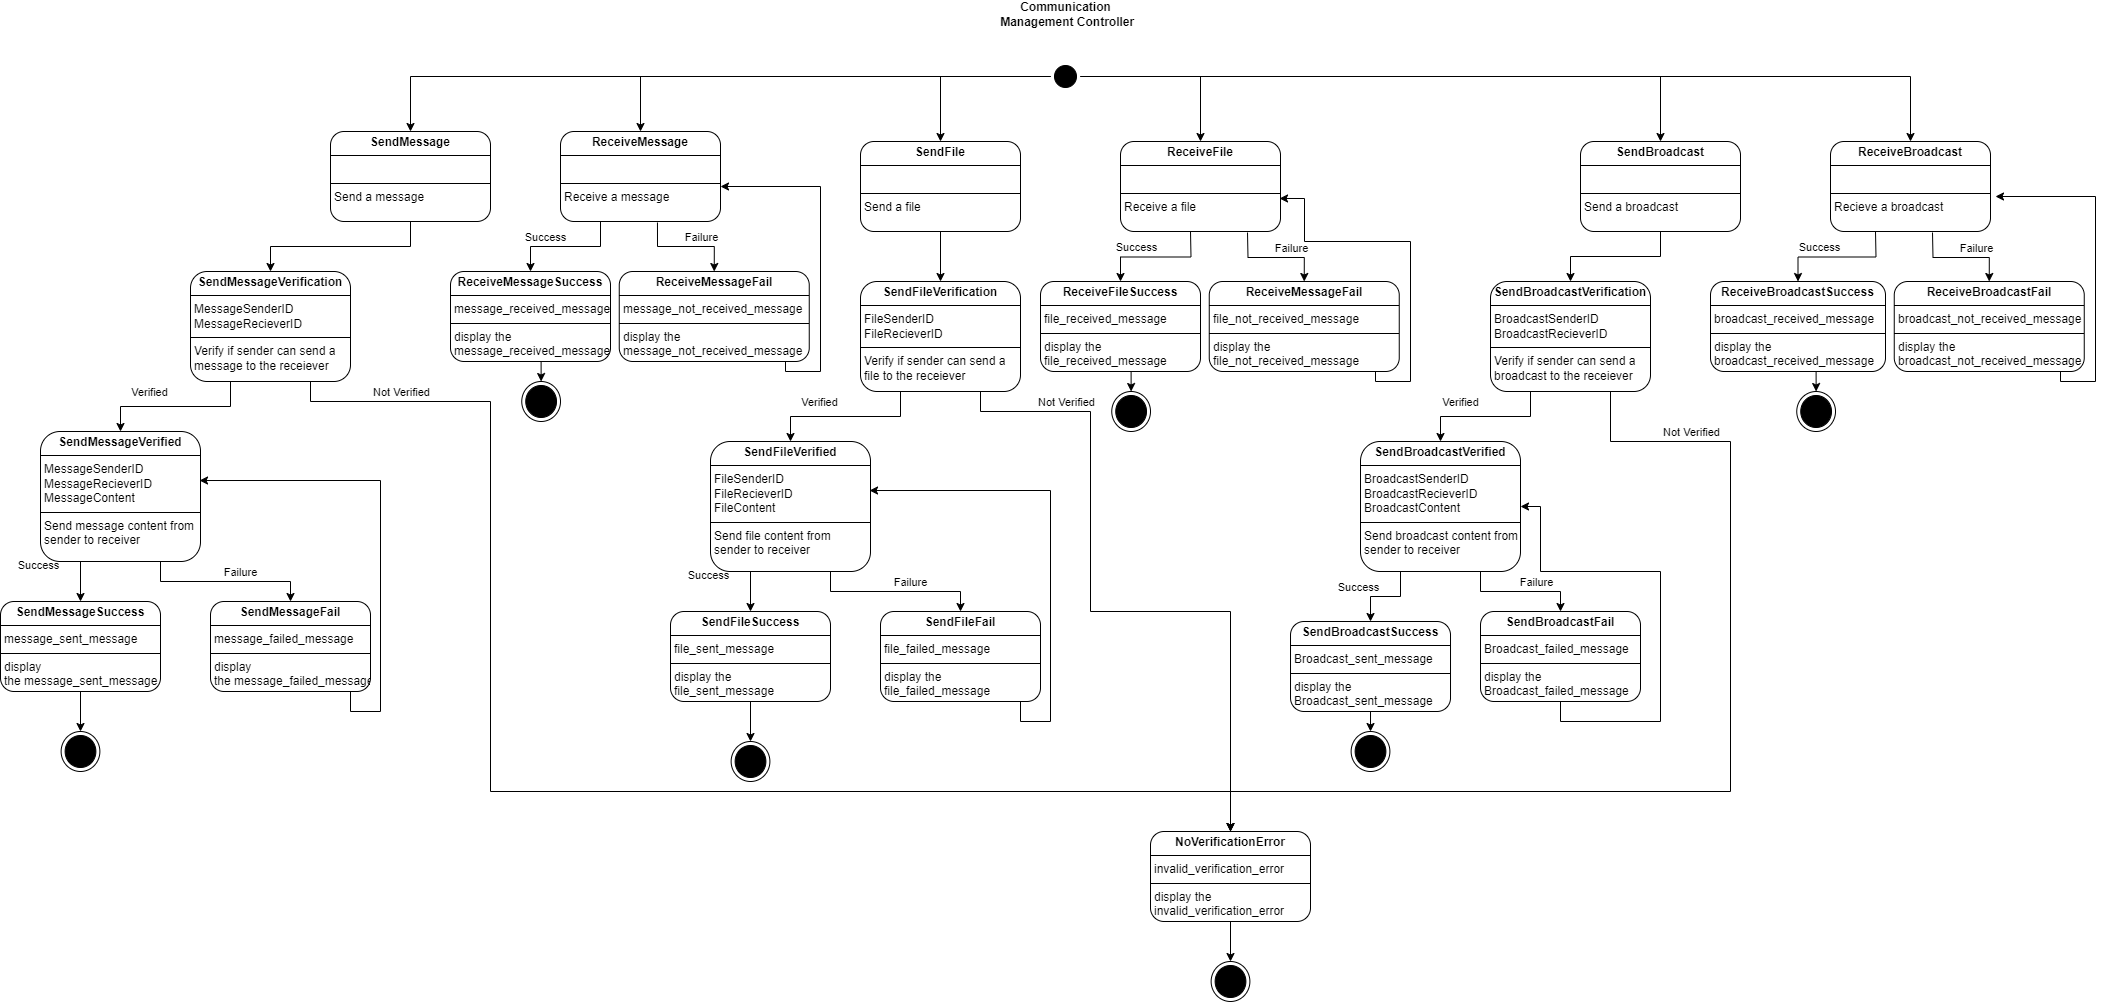
\includegraphics[width=\textwidth]{../images/ControllerStateDiagrams/CommunicationManagementController.drawio.png}
	\textbf{Figure 2.2 Overall Controller Management Controller State Diagram}
	\\A more zoomed in view can be found in figures 2.2.1, 2.2.2, 2.2.3, and 2.2.4.
	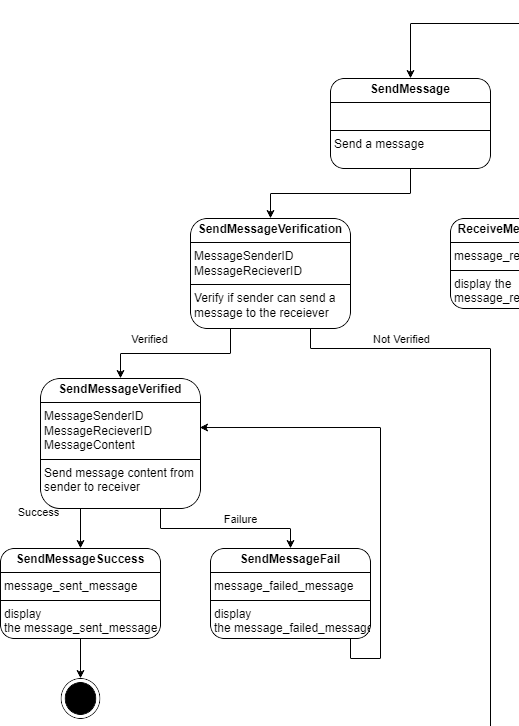
\includegraphics{../images/ControllerStateDiagrams/CMC1.png}\\
	\textbf{Figure 2.2.1 Left of the Controller Management Controller State Diagram}
	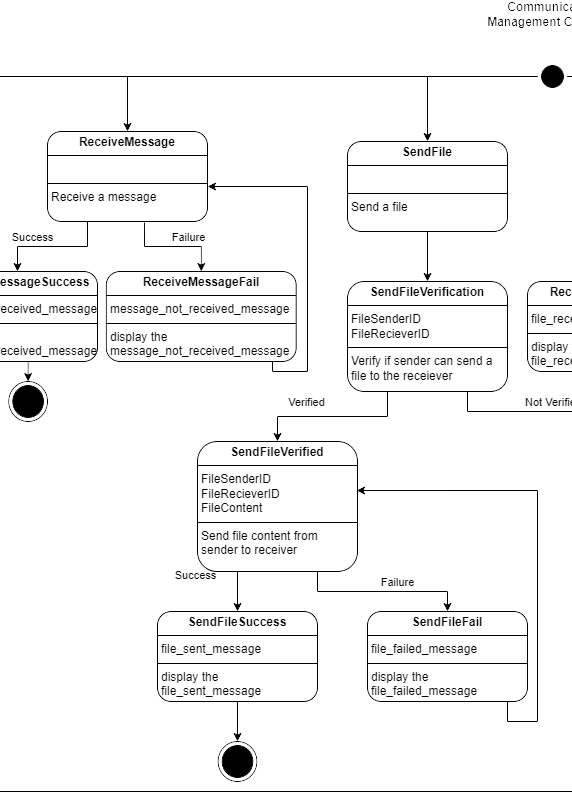
\includegraphics{../images/ControllerStateDiagrams/CMC2.png}\\
	\textbf{Figure 2.2.2 Middle Left of the Controller Management Controller State Diagram}
	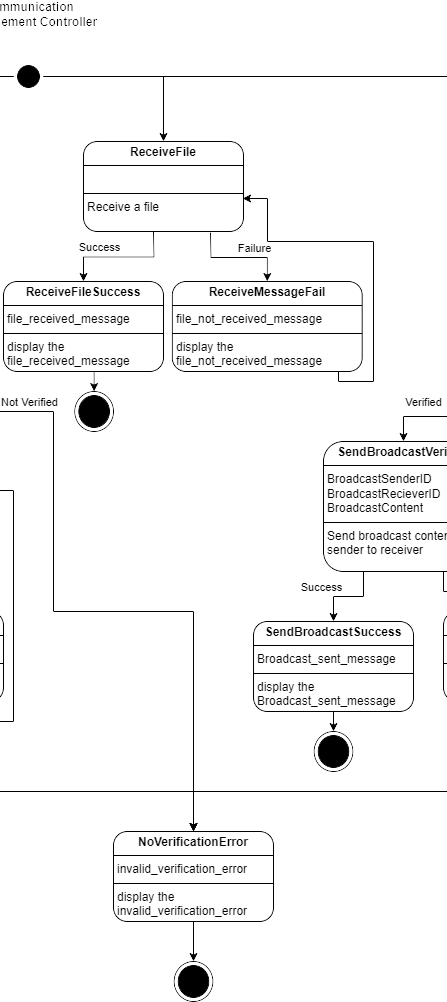
\includegraphics[height=8in]{../images/ControllerStateDiagrams/CMC3.png}\\
	\textbf{Figure 2.2.3 Middle Right of the Controller Management Controller State Diagram}
	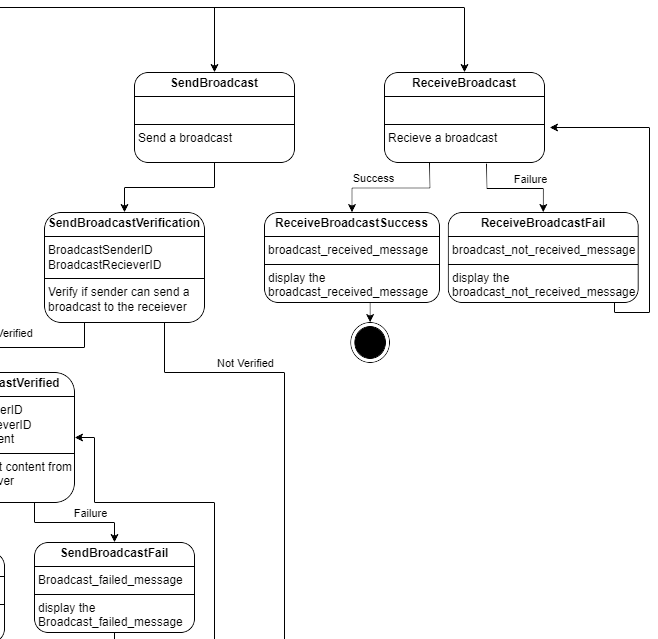
\includegraphics{../images/ControllerStateDiagrams/CMC4.png}\\
	\textbf{Figure 2.2.4 Right of the Controller Management Controller State Diagram}

	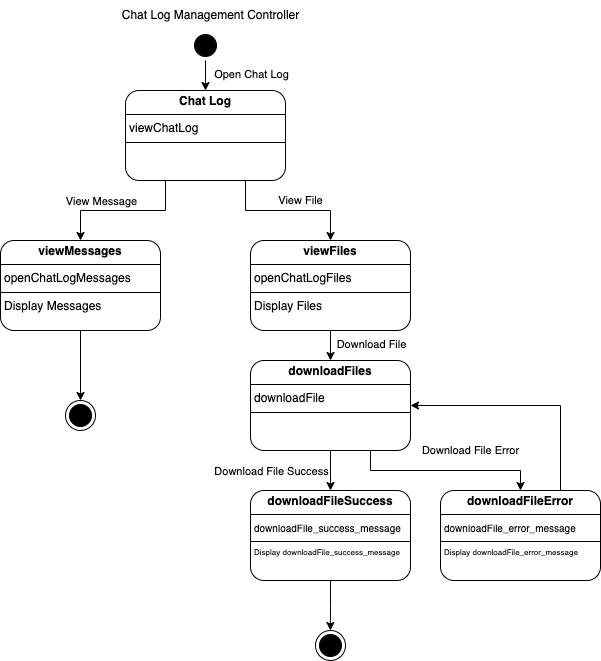
\includegraphics[width=\textwidth]{../images/ControllerStateDiagrams/ChatlogManagement.png}
	\textbf{Figure 2.3 Overall Chat Log Management Controller State Diagram}
	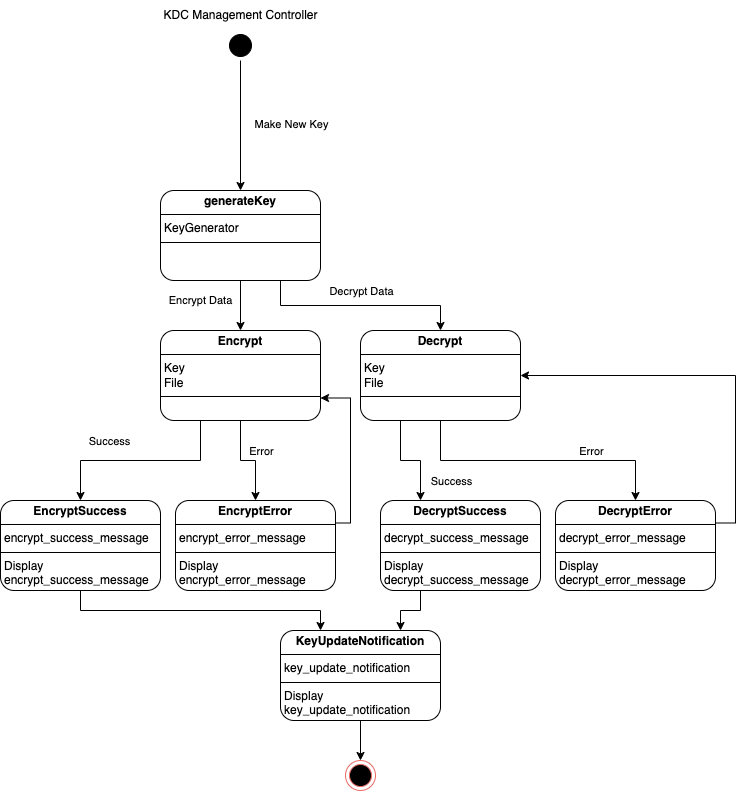
\includegraphics[width=\textwidth]{../images/ControllerStateDiagrams/KDCManagement.png}
	\textbf{Figure 2.4 Overall KDC Management Controller State Diagram}
	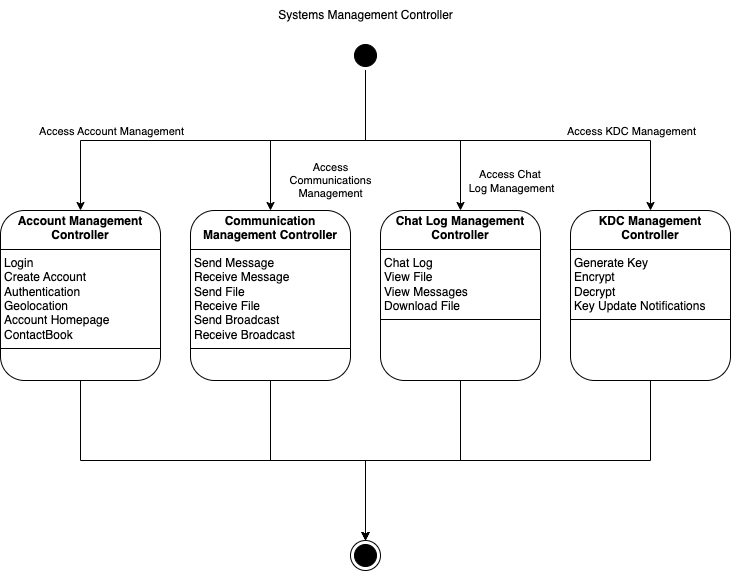
\includegraphics[width=\textwidth]{../images/ControllerStateDiagrams/SystemController.png}
	\textbf{Figure 2.5 Overall System Management Controller State Diagram}
\end{center}

\section{Sequence Diagrams}
\label{sec:sequence_diagrams}
% Begin Section
This section should provide a sequence diagram for each use case of your application.
% End Section
\newpage
\section{Detailed Class Diagram}
\label{sec:detailed_class_diagram}
% Begin Section
This section should provide a detailed class diagram for your application.
\begin{center}
	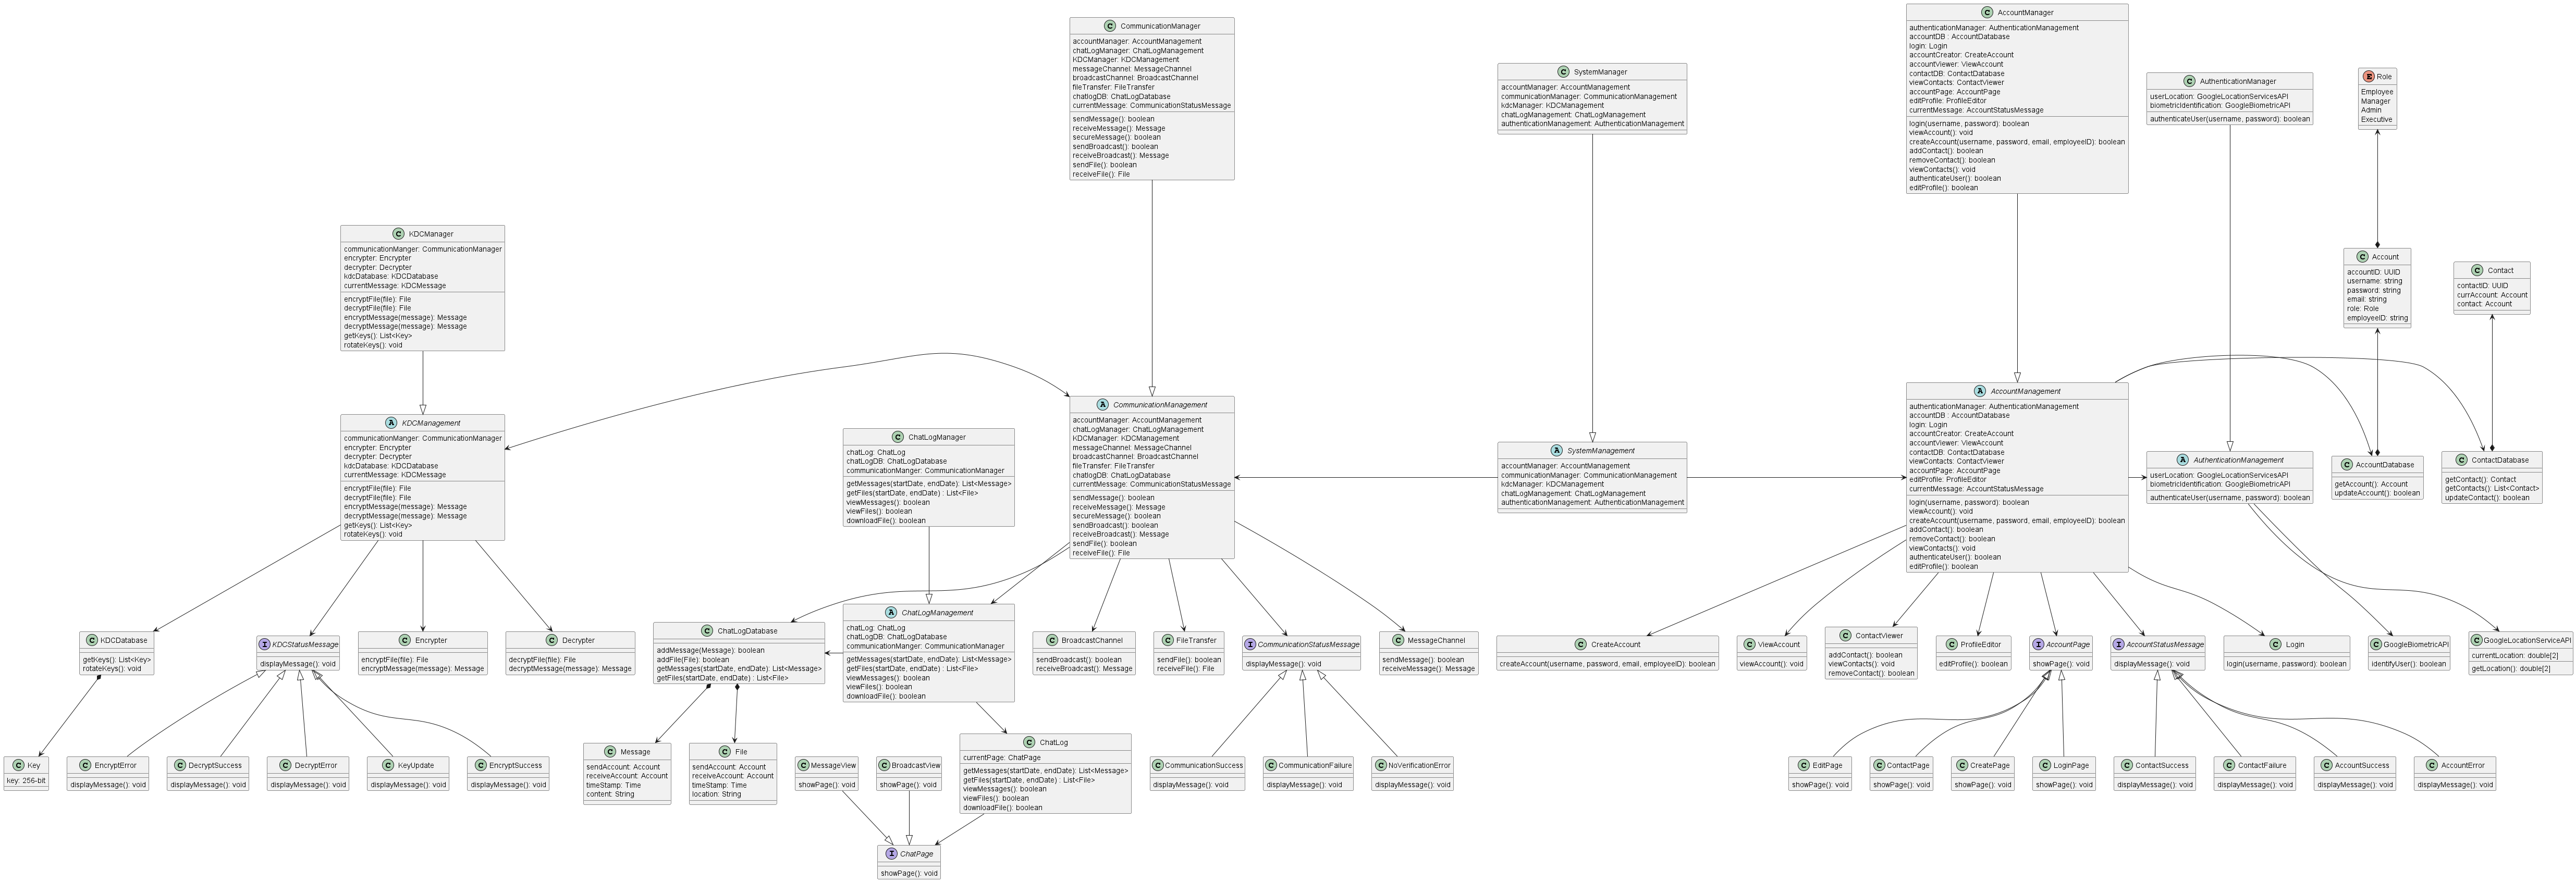
\includegraphics[width=\textwidth]{../images/ClassDiagram/FullClass.png}
	\textbf{Figure 4.1 Overall Detailed Class Diagram}
	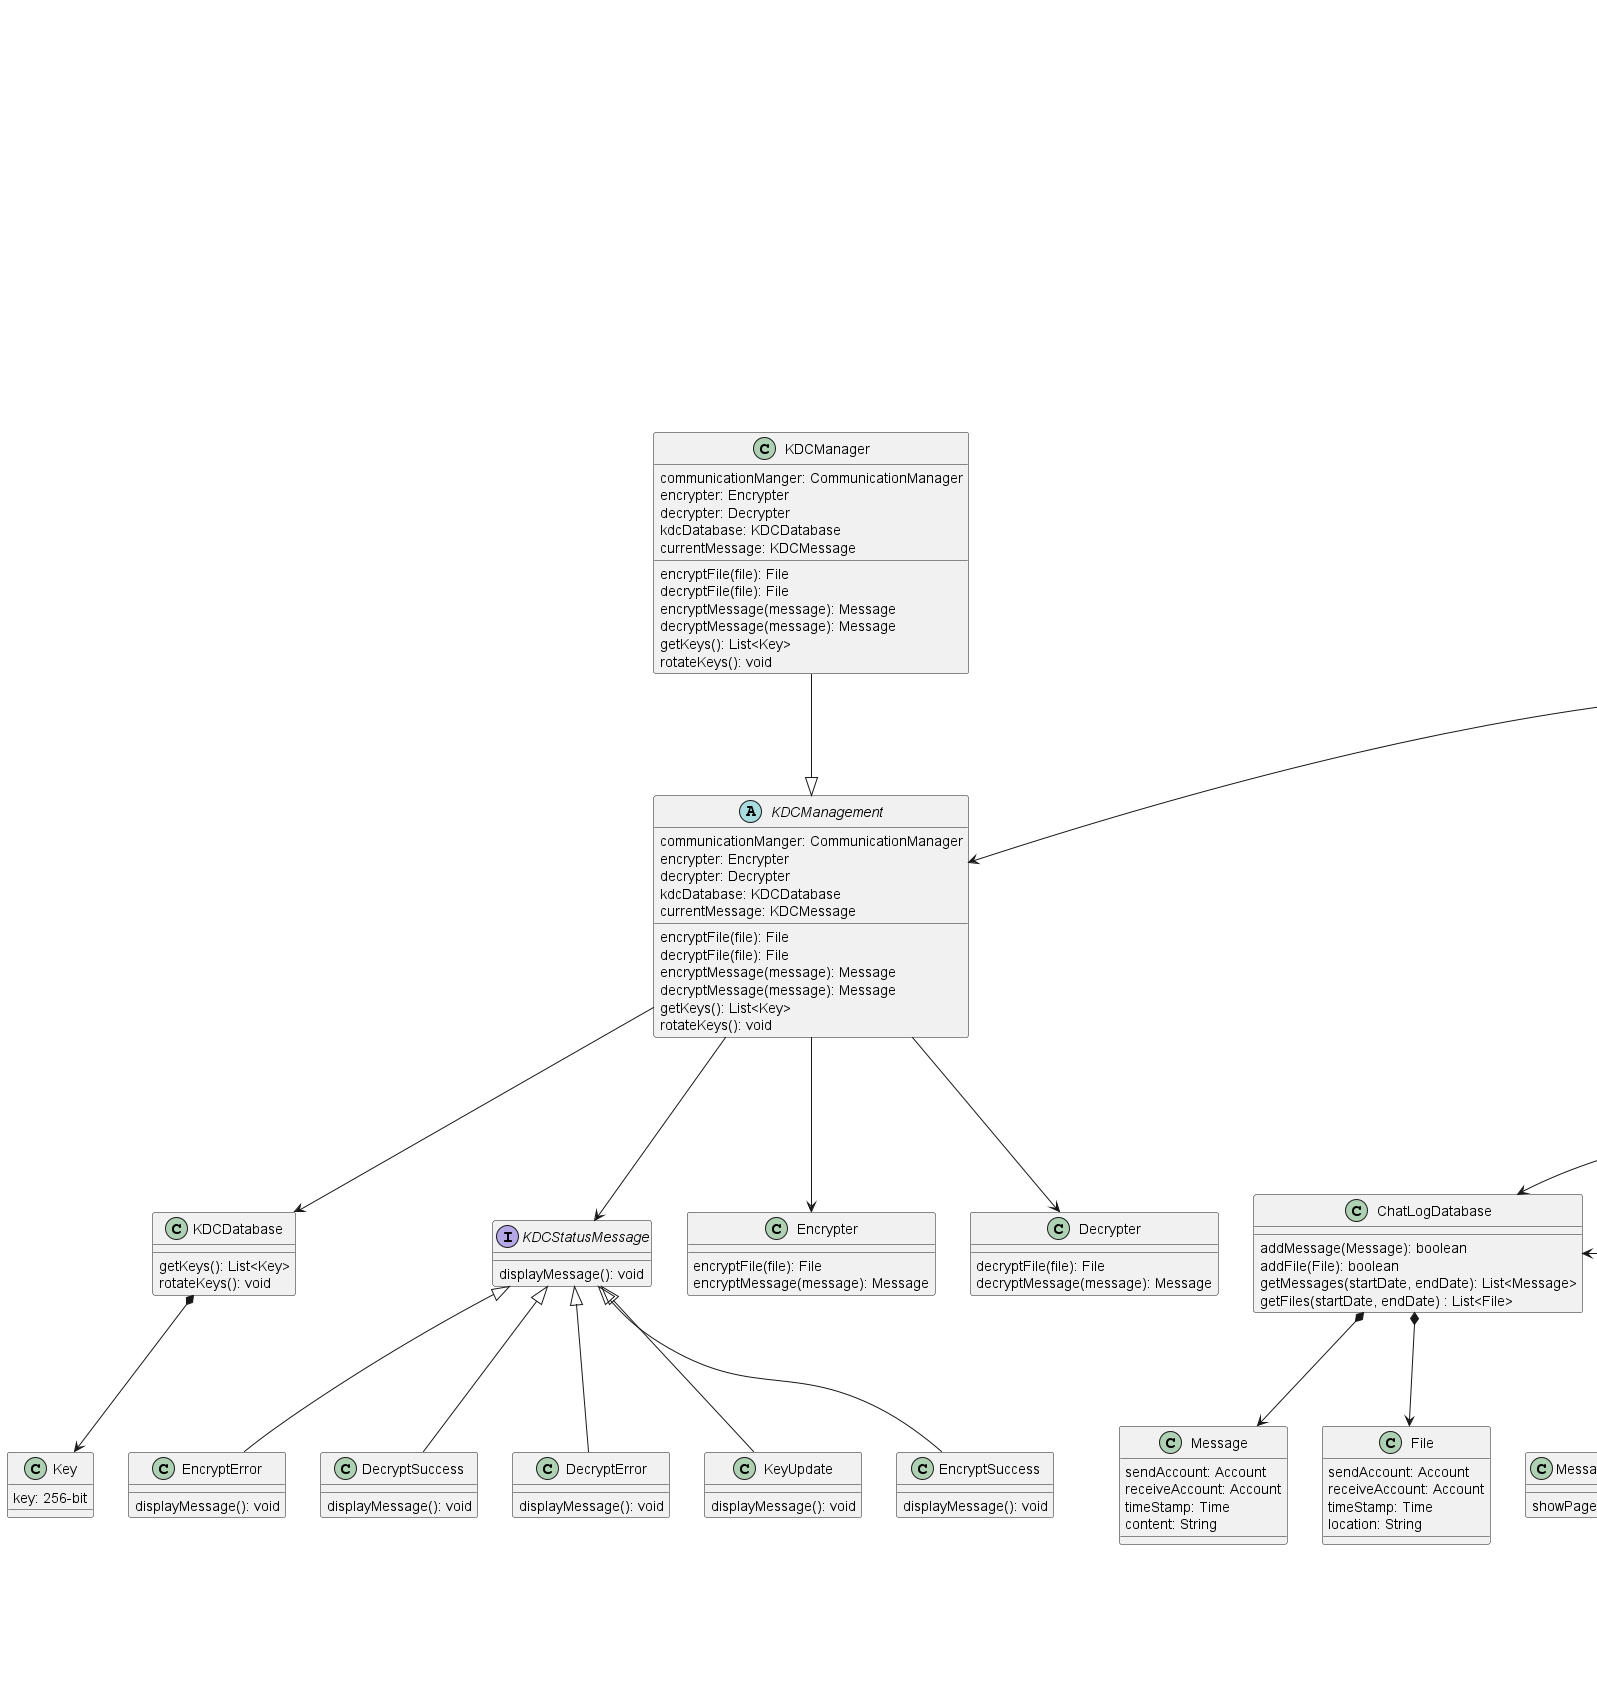
\includegraphics[width=\textwidth,height=8in]{../images/ClassDiagram/left.png}
	\textbf{Figure 4.1.1 Detailed Class Diagram Part 1}
	\newline This is on the far left side of the overall detailed diagram. On its right is figure 4.1.2.
	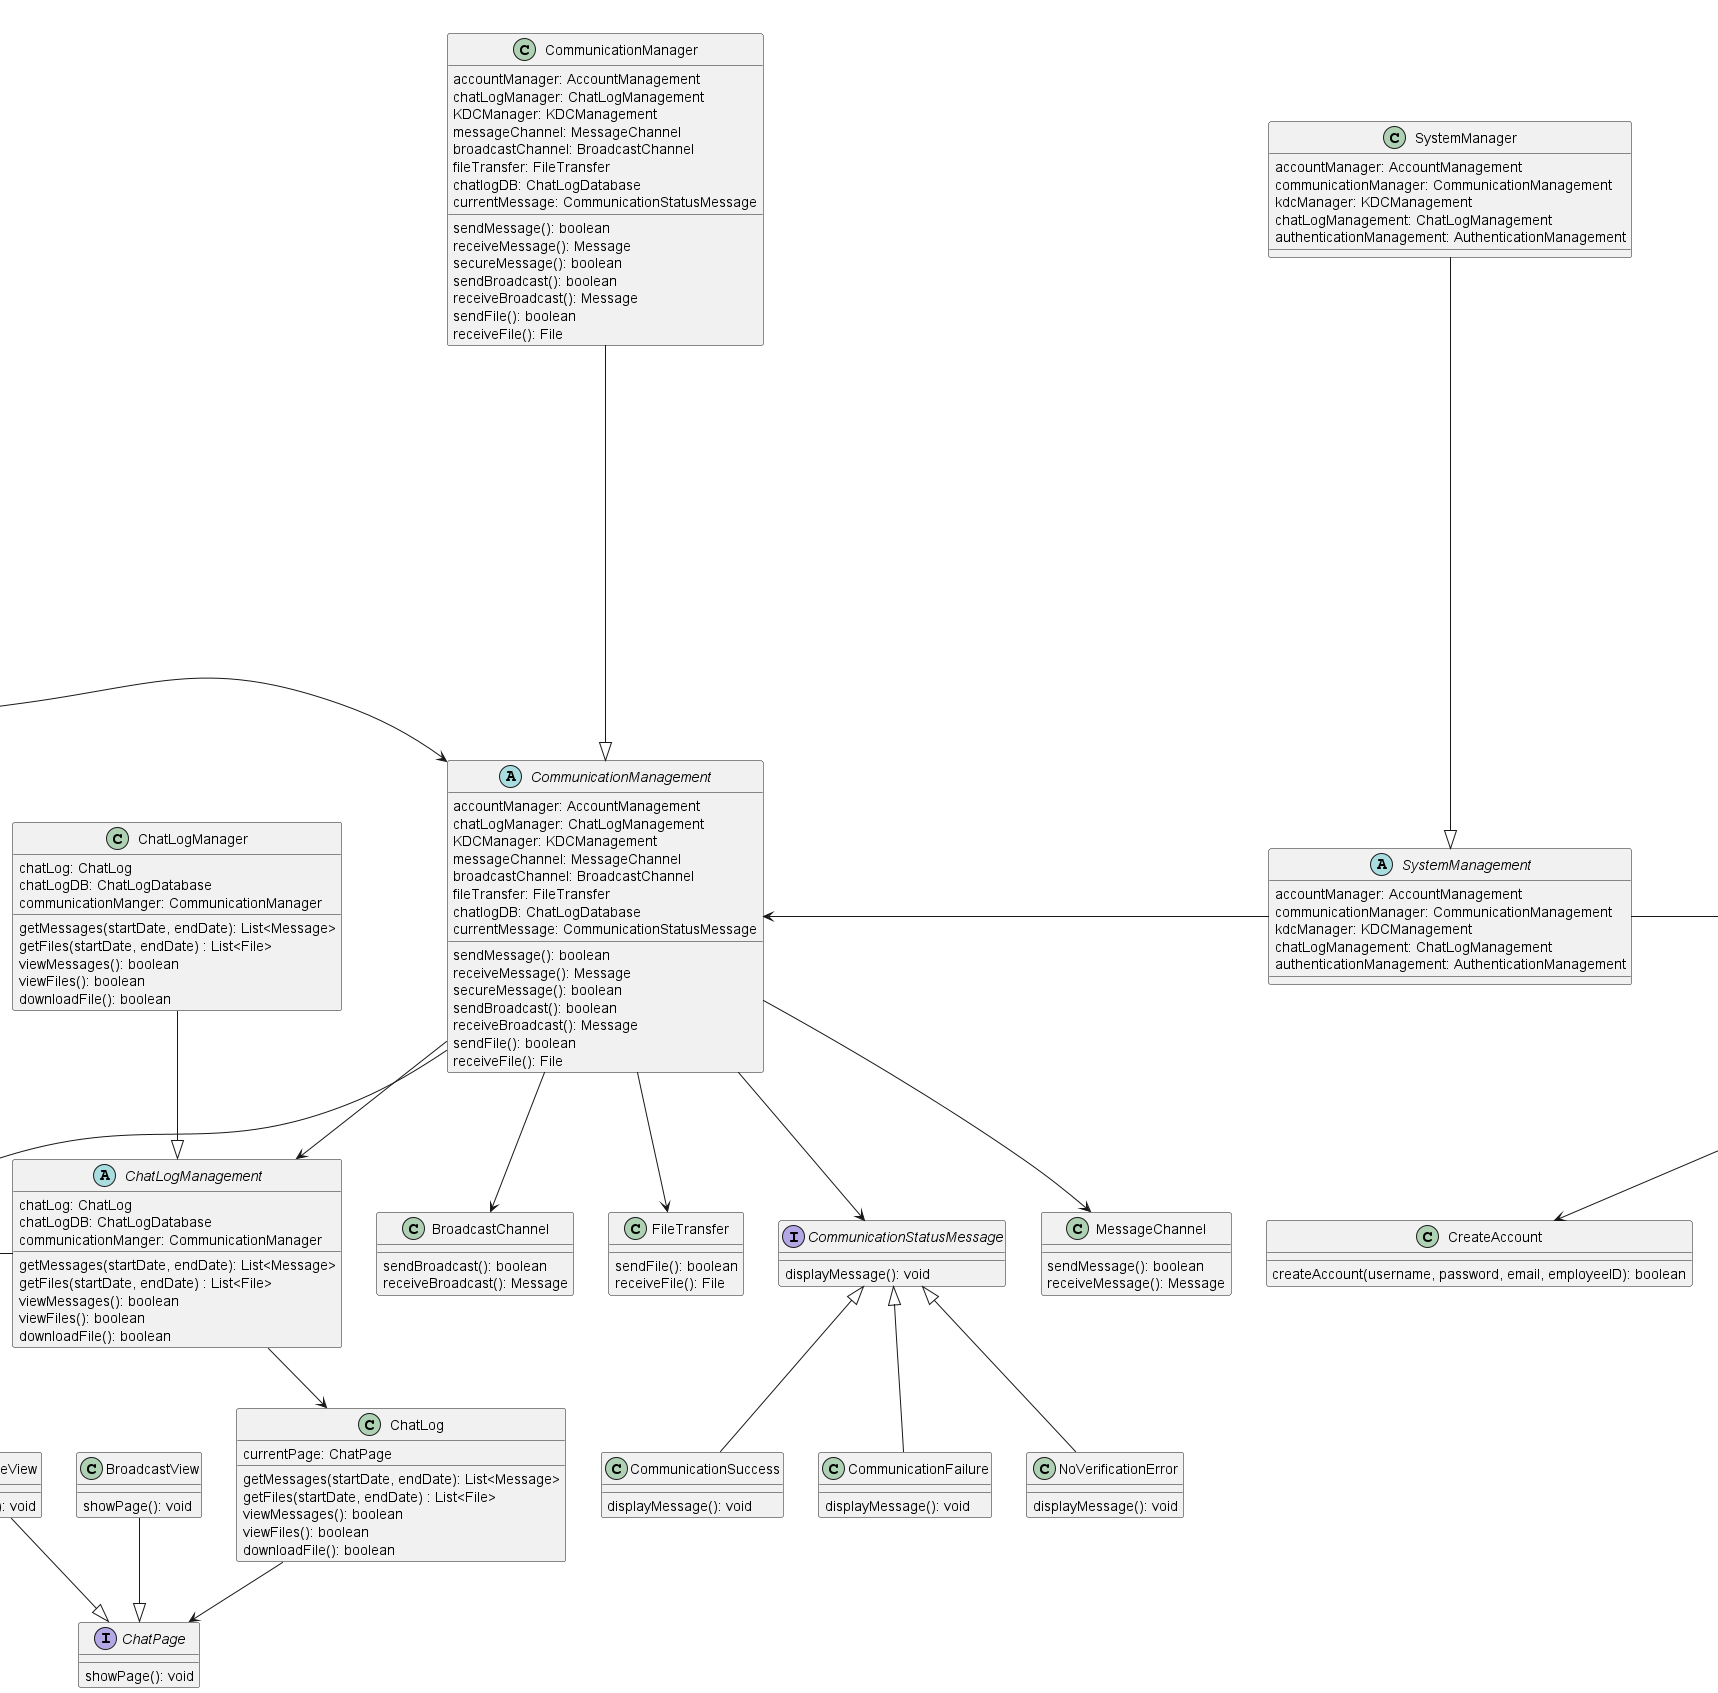
\includegraphics[width=\textwidth,height=8in]{../images/ClassDiagram/mid.png}
	\textbf{Figure 4.1.2 Detailed Class Diagram Part 2}
	\newline This is on the middle of the overall detailed diagram. On its right is figure 4.1.3 and on the left is 4.1.1.
	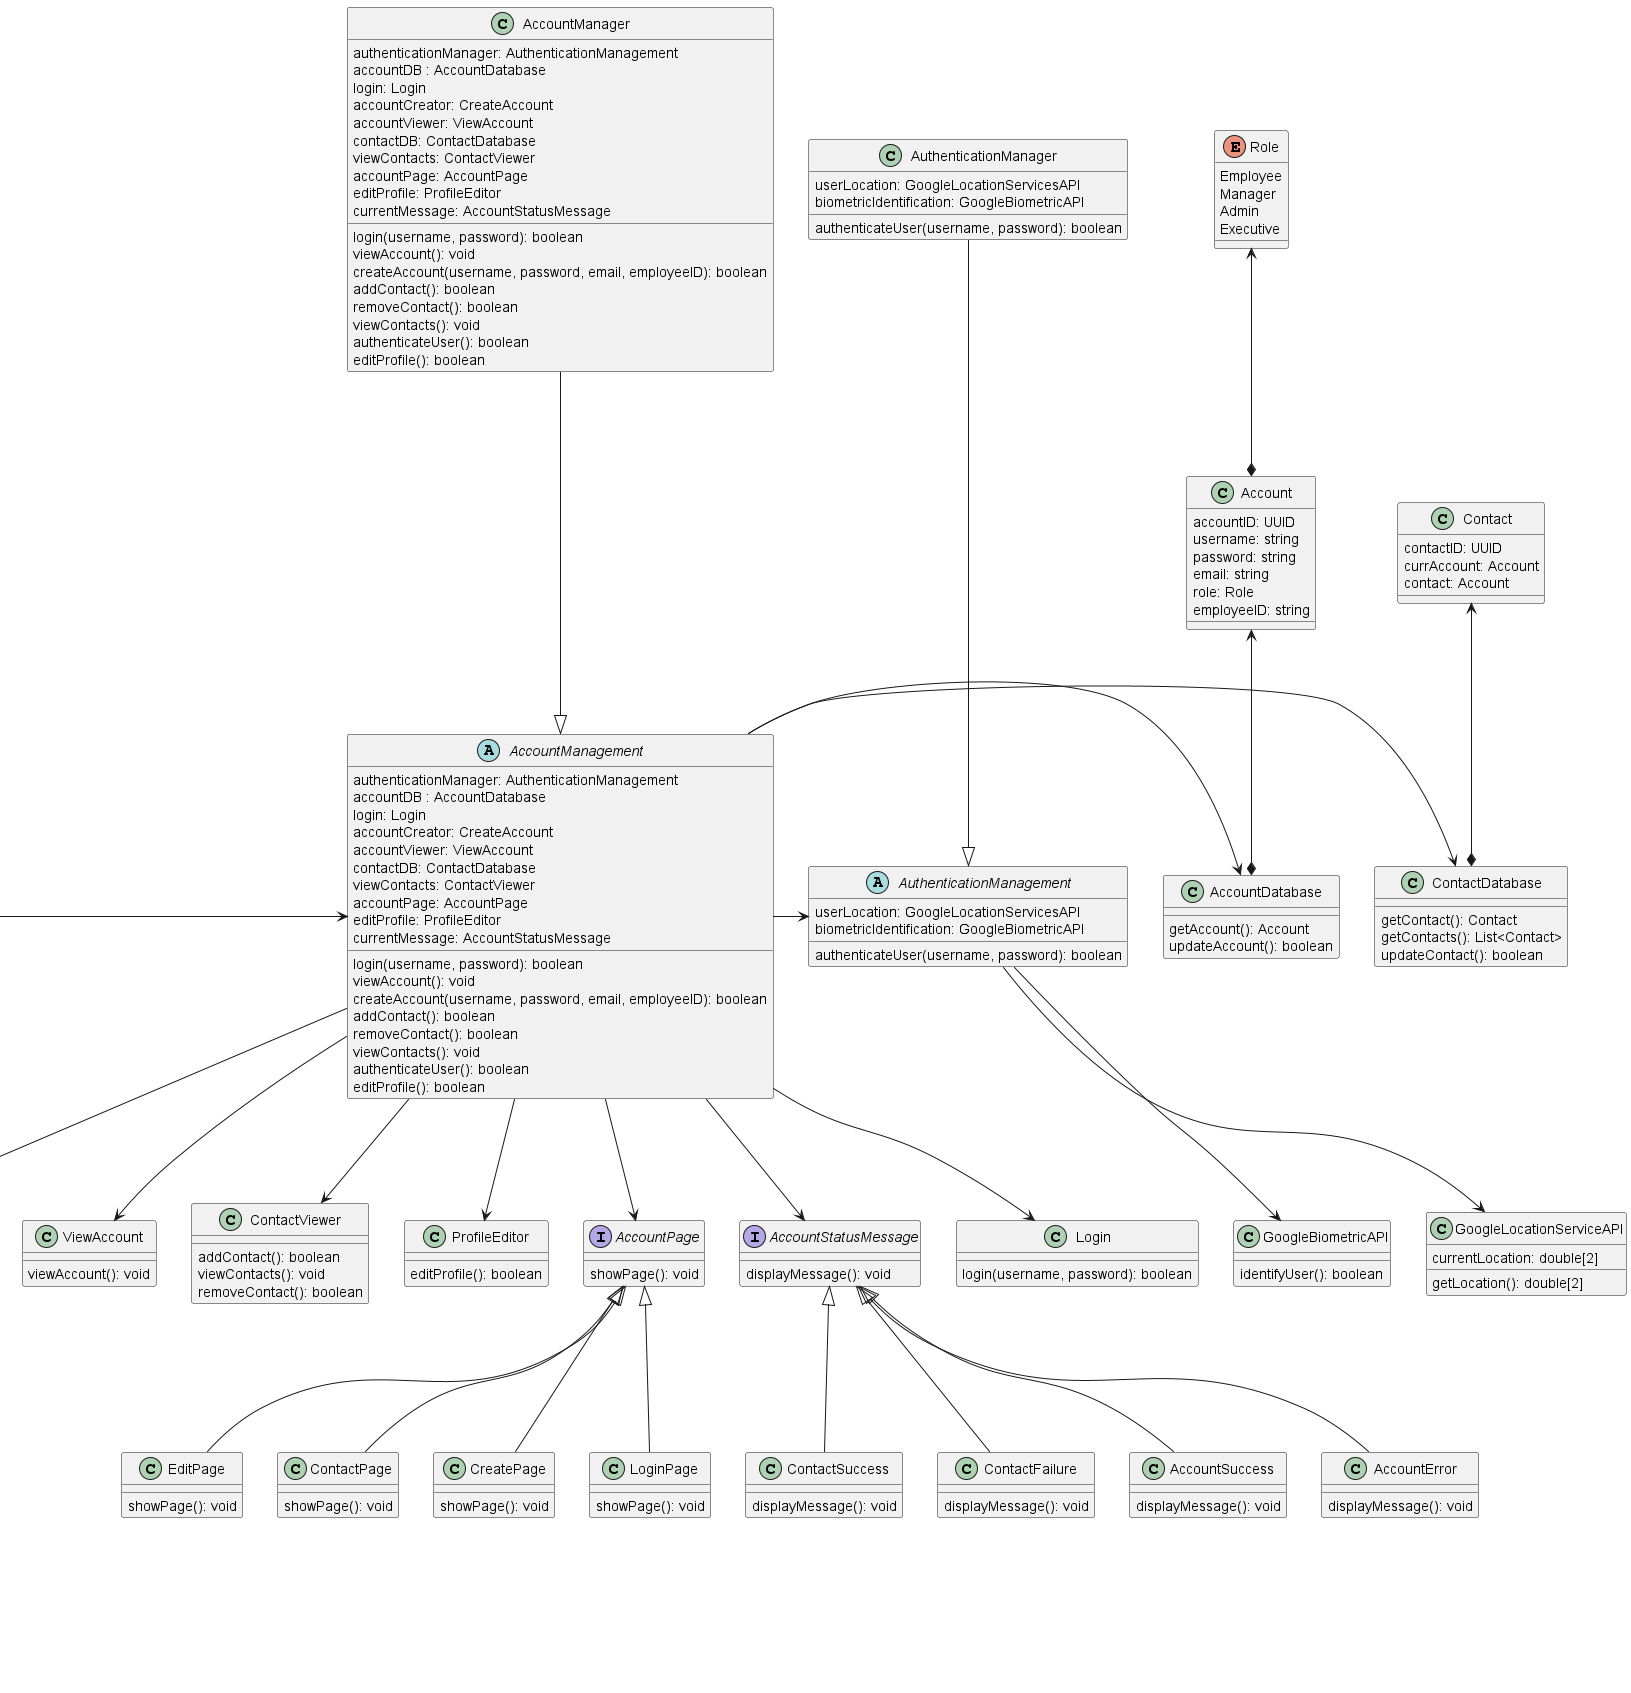
\includegraphics[width=\textwidth,height=8in]{../images/ClassDiagram/right.png}
	\textbf{Figure 4.1.3 Detailed Class Diagram Part 3}
	\newline This is on the far right of the overall detailed diagram. On the left is 4.1.2.
\end{center}
% End Section

\appendix
\section{Division of Labour}
\label{sec:division_of_labour}
% Begin Section
\subsection*{Noah Goldschmied:}
\begin{itemize}
	\item Section 1.1 - Purpose
	\item Section 1.2 - System Description
	\item Section 1.3 - Overview
	\item Figures 2.1, 2.1.1, 2.1.2, 2.1.3 - Account Management Controller State Diagrams
	\item Figures 2.2, 2.2.1, 2.2.2, 2.1.3, 2.1.4 - Communication Management Controller State Diagrams
	\item Reviewed the whole document as a group
\end{itemize}
\begin{figure}[h]
	\centering
	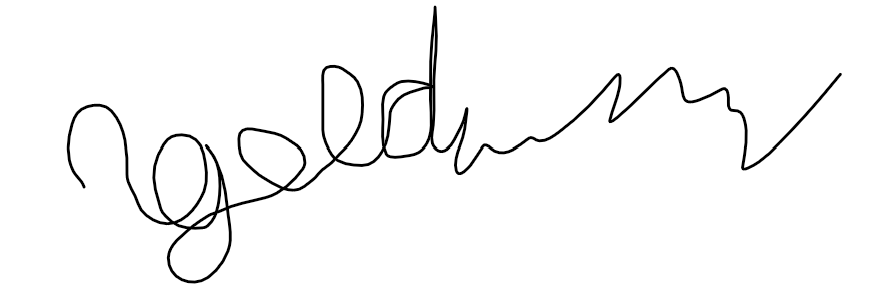
\includegraphics[width=0.5\textwidth]{../images/NoahSignature.png}
	\label{fig:signature}
\end{figure}
\subsection*{Leo Vugert:}
\begin{itemize}
	\item Figures 2.1, 2.1.1, 2.1.2, 2.1.3 - Account Management Controller State Diagrams
	\item Section 2.3 - Chat Log Management Controller State Diagram
	\item Section 2.4 - KDC Management Controller State Diagram
	\item Section 2.5 - System Management Controller State Diagram
	\item Reviewed the whole document as a group
\end{itemize}
\begin{figure}[h]
	\centering
	
\includegraphics[width=0.5\textwidth]{../images/LeoSignature.jpg}
	\label{fig:signature}
\end{figure}
\subsection*{Virochaan Ravichandran Gowri:}
\begin{itemize}
	\item Section 4 - Overall Detailed Class Diagram
	\item Figures 4.1, 4.1.1, 4.1.2, 4.1.3 - Overall Class Diagram as well as subdiagrams.
	\item Reviewed the whole document as a group
\end{itemize}
\begin{figure}[h]
	\centering
	
\includegraphics[width=0.5\textwidth]{../images/ViroSignature.jpg}
	\label{fig:signature}
\end{figure}
\subsection*{Krish Dogra:}
\begin{itemize}
	\item Section 4 - Overall Detailed Class Diagram
	\item Reviewed the whole document as a group
\end{itemize}
\begin{figure}[h]
	\centering
	
\includegraphics[width=0.5\textwidth]{../images/KrishSignature.jpg}
	\label{fig:signature}
\end{figure}
% End Section

\newpage
\section*{IMPORTANT NOTES}
\begin{itemize}
	\item You do \underline{NOT} need to provide a text explanation of each diagram; the diagram should speak for itself
	\item Please document any non-standard notations that you may have used
	      \begin{itemize}
		      \item \emph{Rule of Thumb}: if you feel there is any doubt surrounding the meaning of your notations, document them
	      \end{itemize}
	\item Some diagrams may be difficult to fit into one page
	      \begin{itemize}
		      \item It is OK if the text is small but please ensure that it is readable when printed
		      \item If you need to break a diagram onto multiple pages, please adopt a system of doing so and throughly explain how it can be reconnected from one page to the next; if you are unsure about this, please ask me
	      \end{itemize}
	\item Please submit the latest version of Deliverable 1 and Deliverable 2 with Deliverable 3
	      \begin{itemize}
		      \item They do not have to be a freshly printed versions; the latest marked versions are OK
	      \end{itemize}
	\item If you do \underline{NOT} have a Division of Labour sheet, your deliverable will \underline{NOT} be marked
\end{itemize}


\end{document}
%------------------------------------------------------------------------------